\documentclass[conference]{IEEEtran}
\IEEEoverridecommandlockouts

\usepackage{cite}
\usepackage{amsmath,amssymb}
\usepackage{graphicx}
\usepackage{booktabs}
\usepackage{url}
\usepackage[hidelinks]{hyperref}

\graphicspath{{../figuras/}}

\begin{document}

\title{Linear Regularisation, Latent Projections, and Neural Ensembles for Predicting Aqueous Solubility from Molecular Descriptors}

\newcommand{\autorbloco}[2]{%
  \begin{minipage}[t]{0.46\textwidth}\centering
  {\normalsize #1}\\[0.35em]
  {\small #2\\
  \textit{Dep.\ de Eng.\ de Teleinformática}\\
  \textit{Universidade Federal do Ceará}}
  \end{minipage}}

\author{%
\parbox{\textwidth}{\centering
\autorbloco{Ícaro Adriano}{609310}\hfill\autorbloco{Matheus Reis}{571954}\\[1.4em]
\autorbloco{Alisson Jaime}{555083}\hfill\autorbloco{Vinícius A. G. do Nascimento}{568594}}
}

\maketitle

\begin{abstract}
Predicting aqueous solubility directly from molecular structure is a central regression problem in computational chemistry and early-stage drug discovery. This study evaluates four regression models on a dataset of $1{,}267$ chemical compounds ($951$ training and $316$ test observations) characterised by $228$ collinear molecular descriptors subjected to Yeo-Johnson transformation and standardisation. We implement ordinary least squares (OLS), $L_2$-penalised ridge regression, and partial least squares (PLS) via the NIPALS algorithm from scratch, comparing them against a regularised multilayer perceptron (MLP) ensemble using cross-validation and paired bootstrap resampling. While ridge regression ($\mathrm{RMSE} = 0.7175$, $R^2 = 0.8805$), PLS ($\mathrm{RMSE} = 0.7337$, $R^2 = 0.8750$), and OLS ($\mathrm{RMSE} = 0.7430$, $R^2 = 0.8718$) perform comparably on the test set without statistically significant differences among them, the nonlinear neural network ensemble achieves a test $\mathrm{RMSE}$ of $0.6407$ ($R^2 = 0.9047$), outperforming all linear estimators even after Bonferroni correction.
\end{abstract}

\begin{IEEEkeywords}
aqueous solubility, ordinary least squares, ridge regression, partial least squares, neural networks
\end{IEEEkeywords}

% =====================================================================
% I. INTRODUCTION
% =====================================================================
\section{Introduction}
\label{sec:intro}

Aqueous solubility governs compound bioavailability, membrane permeation, and formulation viability in pharmaceutical development \cite{kuhn2013}. Because experimental assays across large chemical libraries are costly and time-consuming, quantitative structure-property relationship (QSPR) models seek to estimate logarithmic solubility directly from numerical molecular descriptors. In statistical learning terms, this constitutes a supervised multivariate regression problem in which a continuous response $y \in \mathbb{R}$ is approximated from a predictor vector $\mathbf{x} \in \mathbb{R}^{D}$.

Chemical descriptor matrices present two classical challenges for regression estimators: severe skewness in topological counts and near-exact multicollinearity among structural fingerprints \cite{hastie2009}. Unregularised ordinary least squares (OLS) yields unbiased linear predictions under standard Gauss-Markov assumptions, but its coefficient variance inflates rapidly as singular values of the design matrix approach zero \cite{golub2013}. Two distinct linear strategies address this ill-conditioning: continuous shrinkage via $L_2$ regularisation (ridge regression) \cite{hoerl1970} and supervised dimension reduction onto orthogonal latent factors via partial least squares (PLS). However, linear projections cannot capture higher-order interactions among functional groups unless nonlinear mappings, such as feedforward neural networks, are introduced.

In this work, we implement OLS, ridge regression, and PLS from scratch, verify their numerical agreement against reference implementations \cite{pedregosa2011}, and compare their generalisation capacity against a regularised multilayer perceptron (MLP) ensemble. Section~\ref{sec:methods} details the dataset pre-processing, mathematical formulations, and resampling protocols; Section~\ref{sec:results} presents the cross-validation profiles, test-set predictions, and paired bootstrap comparisons; and Section~\ref{sec:conclusion} summarises our findings.

% =====================================================================
% II. METHODS
% =====================================================================
\section{Methods}
\label{sec:methods}

\subsection{Dataset and pre-processing}
\label{subsec:dataset}

The data are the solubility set distributed with \cite{kuhn2013}, with
$N = 1{,}267$ chemical compounds split into $951$ training and $316$
test observations. Each compound is described by $D = 228$ predictors:
208 binary fingerprints, 16 count descriptors and 4 continuous
descriptors. The outcome is the log solubility of the compound.

All 20 non-binary predictors are right-skewed, so they receive a
Yeo-Johnson transformation \cite{yeo2000}; the binary predictors are
left unchanged. Every predictor is then centred and scaled to unit
standard deviation. The transformation parameters, means and standard
deviations are estimated on the fitting data only and re-applied,
without re-estimation, to the data being evaluated. The transformed
predictors are strongly collinear: 47 pairs have $|r| > 0.9$, and
\texttt{FP134} and \texttt{NumSulfer} are nearly duplicates
($r = 1.000$ to three decimals).

\subsection{Ordinary least squares}
\label{subsec:ols}

With $\mathbf{X}$ centred on the fitting data and
$\mathbf{y}_c = \mathbf{y} - \bar{y}$, the intercept equals $\bar{y}$
and the ordinary least squares (OLS) coefficients are
\begin{equation}
\hat{\boldsymbol{\beta}} =
(\mathbf{X}^{\top}\mathbf{X})^{+}\mathbf{X}^{\top}\mathbf{y}_c =
\mathbf{X}^{+}\mathbf{y}_c,
\label{eq:ols}
\end{equation}
where $(\cdot)^{+}$ is the Moore-Penrose pseudoinverse
\cite{golub2013}. The estimator was implemented from scratch through
the singular value decomposition
$\mathbf{X} = \mathbf{U}\mathbf{S}\mathbf{V}^{\top}$, discarding
singular values below $\max(n,p)\,\varepsilon\,s_{\max}$. Working on
$\mathbf{X}$ avoids squaring its condition number, and the
pseudoinverse returns the minimum-norm solution when the rank drops.
OLS has no tuning parameter and is directly interpretable, but its
coefficients become unstable under collinearity \cite{hastie2009}.

\subsection{Ridge regression}
\label{subsec:ridge}

Ridge regression \cite{hoerl1970} penalises the squared norm of the
coefficients and leaves the intercept unpenalised. With the same
centring, the solution is
\begin{equation}
\hat{\boldsymbol{\beta}}(\lambda) =
(\mathbf{X}^{\top}\mathbf{X} + \lambda\mathbf{I})^{-1}
\mathbf{X}^{\top}\mathbf{y}_c =
\mathbf{V}\,\mathrm{diag}\!\left(\frac{s_i}{s_i^{2}+\lambda}\right)
\mathbf{U}^{\top}\mathbf{y}_c.
\label{eq:ridge}
\end{equation}
The form on the right, also implemented from scratch, needs a single
decomposition for the whole search. The penalty shrinks the directions
of small singular value and so stabilises the coefficients, at the cost
of a bias and of having to select $\lambda$. We search 29 values spaced
logarithmically between $10^{-3}$ and $10^{4}$ and take the value that
minimises the mean cross-validated RMSE.

\subsection{Resampling and performance measures}
\label{subsec:cv}

Cross-validation uses the training set only, in 10 folds of 95 or 96
compounds drawn with a fixed seed and shared by the OLS, ridge, and PLS
analyses. In each fold, the pre-processing and the model are estimated
on the other nine folds and applied to the held-out fold. Performance
is measured by $\mathrm{RMSE}$ and by
$R^2 = 1 - \mathrm{SSE}/\mathrm{SST}$, averaged over the folds, with
the standard error of the mean. Both the models and the cross-validation
were compared with \texttt{LinearRegression}, \texttt{Ridge},
\texttt{cross\_validate} and \texttt{GridSearchCV} from scikit-learn
\cite{pedregosa2011}, with the pre-processing placed inside a
\texttt{Pipeline} to preserve the separation between folds. Test-set
uncertainty is expressed by $95\%$ percentile bootstrap intervals
\cite{efron1993} over 5000 resamples of the 316 test compounds.

\subsection{Partial least squares and neural network}
\label{subsec:pls-nn}

Partial least squares (PLS) constructs $A \le D$ orthogonal latent
scores $\mathbf{t}_a = \mathbf{X}_{a-1}\mathbf{w}_a$ that maximise the
sample covariance with the deflated response \cite{hastie2009}. We
implemented the univariate NIPALS algorithm from scratch: at step $a$,
weights $\mathbf{w}_a = \mathbf{X}_{a-1}^{\top}\mathbf{y}_{a-1} /
\|\mathbf{X}_{a-1}^{\top}\mathbf{y}_{a-1}\|_2$ produce scores
$\mathbf{t}_a$, loadings $\mathbf{p}_a =
\mathbf{X}_{a-1}^{\top}\mathbf{t}_a / (\mathbf{t}_a^{\top}\mathbf{t}_a)$,
and response weights $q_a = \mathbf{y}_{a-1}^{\top}\mathbf{t}_a /
(\mathbf{t}_a^{\top}\mathbf{t}_a)$, followed by rank-one deflation of
$\mathbf{X}_{a-1}$ and $\mathbf{y}_{a-1}$. Accumulating $A$ components
yields the direct regression vector $\hat{\boldsymbol{\beta}}_{\mathrm{PLS}}(A) =
\mathbf{W}(\mathbf{P}^{\top}\mathbf{W})^{-1}\mathbf{q}$. We evaluate
$A \in \{1,\dots,40\}$ via 10-fold CV. PLS handles collinearity via
supervised projection and reduces dimensionality, though latent factors
mix all original descriptors.

To capture nonlinear interactions, we train feedforward multilayer
perceptrons (MLPs) with ReLU activations, dropout, and $L_2$ weight
decay using AdamW ($\eta = 10^{-3}$, batch size $64$) on standardised
targets. Because neural networks are sensitive to hyperparameter choices
and random weight initialisation, we perform a 5-fold cross-validation
grid search over architectures $\{(16,), (64,), (128,), (64, 32)\}$,
weight decay $\{10^{-2}, 10^{-1}, 1.0\}$, dropout $\{0.0, 0.3\}$, and
training epochs from $25$ to $300$ in steps of $25$. The final predictor averages
an ensemble of $5$ independently initialised networks trained on the full
training set under the selected configuration, reducing variance at the
cost of higher computational effort and lower interpretability.

% =====================================================================
% III. RESULTS
% =====================================================================
\section{Results and Discussion}
\label{sec:results}

\subsection{Ordinary least squares}
\label{subsec:res-ols}

Table~\ref{tab:ols} summarises the OLS results. On the full training
set $\mathbf{X}$ has numerical rank $228$ of $228$ and a condition
number of about $3.1 \times 10^{4}$: it is badly conditioned but not
exactly singular. The collinearity is visible in the coefficients.
\texttt{NumSulfer} receives $-106.14$ and \texttt{FP134} receives
$+105.95$, two values that nearly cancel, so that only their sum is
well determined by the data.

\begin{table}[htbp]
\caption{OLS performance. CV values are the mean over 10 folds
$\pm$ the standard error; the test interval is a $95\%$ bootstrap
interval.}
\label{tab:ols}
\centering
\begin{tabular}{lll}
\toprule
Set & RMSE & $R^2$ \\
\midrule
Training & $0.4900$ & $0.9426$ \\
10-fold CV & $0.7279 \pm 0.0215$ & $0.8654 \pm 0.0128$ \\
Test & $0.7430$ & $0.8718$ \\
Test interval & $[0.6645,\ 0.8243]$ & $[0.8327,\ 0.9027]$ \\
\bottomrule
\end{tabular}
\end{table}

The implementation agrees with scikit-learn to numerical precision. On
the test set both give an RMSE of $0.742978$ and an $R^2$ of
$0.871814$, with a largest difference of $1.5 \times 10^{-10}$ in the
coefficients and of $5.4 \times 10^{-13}$ in the predictions. The two
cross-validations differ by at most $1.3 \times 10^{-11}$ in the RMSE
of any fold. In folds 4 and 7 the rank falls to $227$, since removing
some compounds makes one column an exact combination of the others;
this is where the pseudoinverse of \eqref{eq:ols} is indispensable.

The gap between the training RMSE of $0.4900$ and the test RMSE of
$0.7430$ indicates overfitting, with 228 coefficients estimated from
951 compounds. Cross-validation anticipated the test performance well,
as Fig.~\ref{fig:ols} shows. The test RMSE lies $0.0151$ above the CV
mean, less than one standard error, and inside the $95\%$ interval of
the CV mean, $[0.679,\ 0.777]$. The test $R^2$ likewise lies inside the
corresponding interval, $[0.837,\ 0.894]$. The RMSE of individual folds
ranges from $0.611$ to $0.853$, and the test points follow the diagonal
across the whole solubility range.

\begin{figure}[htbp]
\centering
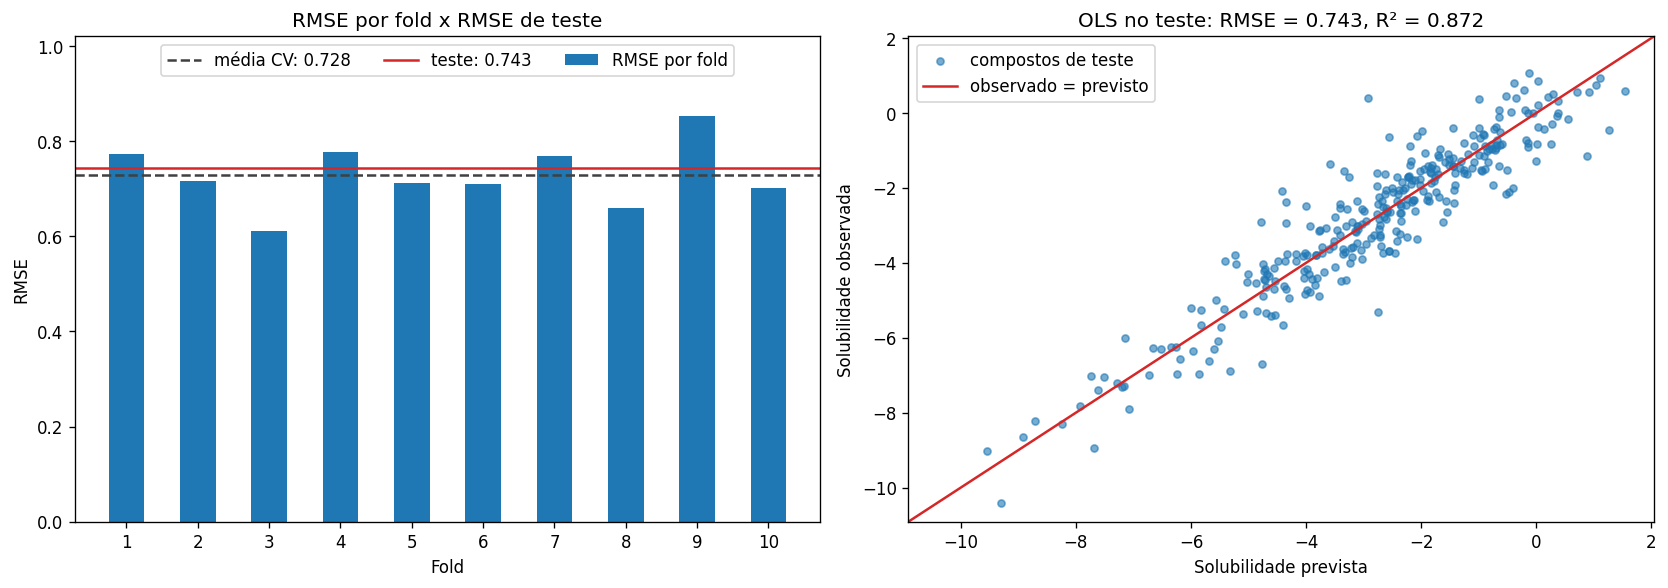
\includegraphics[width=\columnwidth]{ols_cv_vs_teste.png}
\caption{OLS: RMSE per fold against the CV mean and the test RMSE
(left), and observed against predicted solubility on the test set
(right).}
\label{fig:ols}
\end{figure}

\subsection{Ridge regression}
\label{subsec:res-ridge}

The solution of \eqref{eq:ridge} matches the normal equations written
with an explicit unpenalised intercept to within $7.1 \times 10^{-14}$,
and the intercept obtained is exactly $\bar{y}$. Across the 29 values
of $\lambda$ it also matches scikit-learn, with largest differences of
$7.4 \times 10^{-9}$ in the coefficients, at $\lambda = 10^{-3}$, and
of $1.2 \times 10^{-11}$ in the training predictions.

Fig.~\ref{fig:ridge} shows the cross-validation profile. For small
$\lambda$ the RMSE is that of OLS ($0.7278$). It rises slightly to about
$0.735$ near $\lambda = 0.1$, falls to its minimum at
$\lambda \approx 31.6$, and then grows quickly to $1.3865$ at
$\lambda = 10^{4}$, where the model is over-penalised. The minimum lies
inside the grid, so the search range was sufficient. GridSearchCV
selects the same $\lambda$, with a largest difference in the profiles
of $3.4 \times 10^{-4}$ in the RMSE. This difference has an identified
cause: \texttt{StandardScaler} divides by $n$ and our pre-processing by
$n-1$. Rescaling the columns does not change the OLS predictions, but
in ridge it is equivalent to a slight change of $\lambda$. Under the
same convention the difference falls to $1.1 \times 10^{-13}$.

\begin{figure}[htbp]
\centering
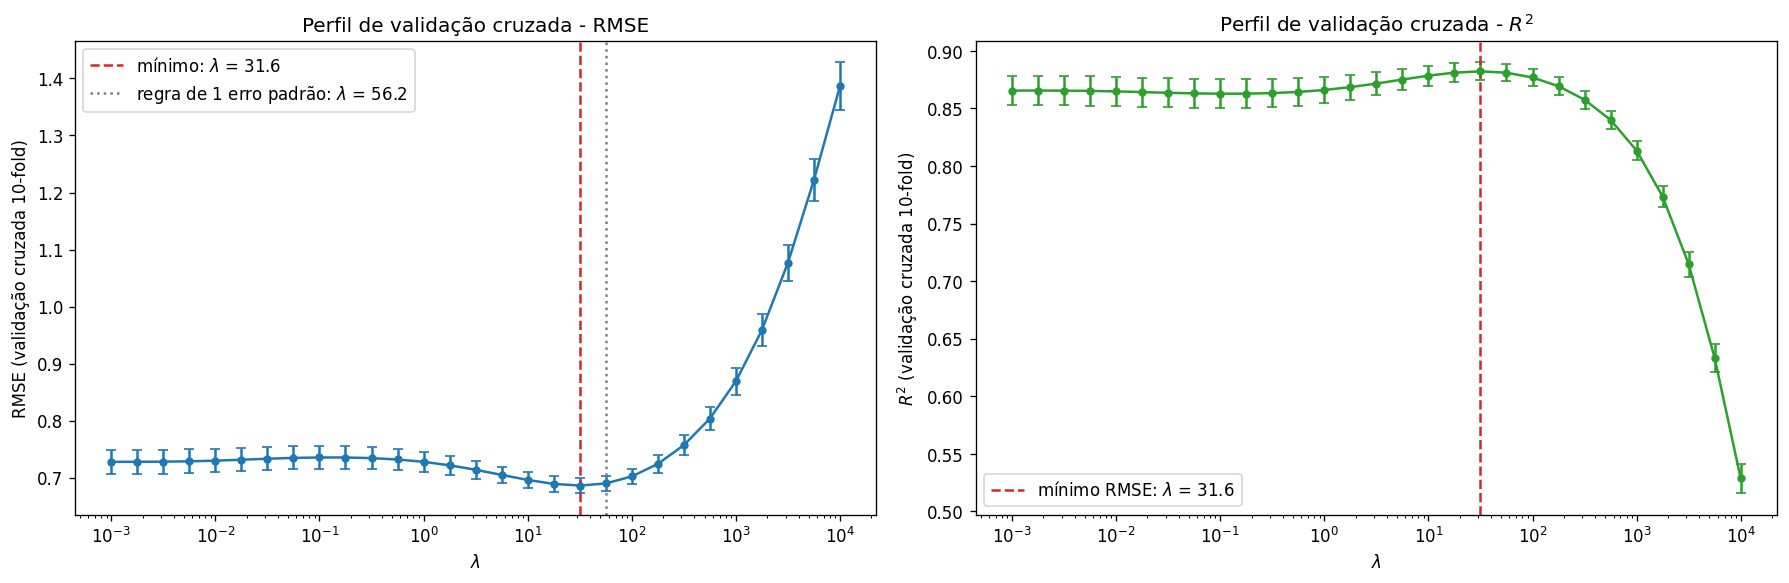
\includegraphics[width=\columnwidth]{ridge_perfil_cv.png}
\caption{Ridge cross-validation profile of RMSE (left) and $R^2$
(right), with the standard error of the mean over 10 folds.}
\label{fig:ridge}
\end{figure}

Table~\ref{tab:ridge} reports the final model, refitted on the whole
training set. Scikit-learn gives the same test result, with a largest
difference of $4.6 \times 10^{-14}$ in the predictions. Relative to
OLS, the penalty reduced the test RMSE by $0.0255$ and the norm of the
coefficients from $152.02$ to $1.48$. The collinear pair is the
clearest case: \texttt{NumSulfer} and \texttt{FP134} become $-0.057$
and $-0.056$, sharing the weight between two nearly duplicate
predictors instead of opposing it.

\begin{table}[htbp]
\caption{Ridge performance with $\lambda \approx 31.6$. CV values are
the mean over 10 folds $\pm$ the standard error; the test interval is a
$95\%$ bootstrap interval.}
\label{tab:ridge}
\centering
\begin{tabular}{lll}
\toprule
Set & RMSE & $R^2$ \\
\midrule
Training & $0.5438$ & $0.9293$ \\
10-fold CV & $0.6862 \pm 0.0131$ & $0.8822 \pm 0.0077$ \\
Test & $0.7175$ & $0.8805$ \\
Test interval & $[0.6457,\ 0.7898]$ & $[0.8466,\ 0.9074]$ \\
\bottomrule
\end{tabular}
\end{table}

The cross-validated estimate is more optimistic than for OLS: the CV
RMSE lies $0.0313$ below the test RMSE, about 2.4 standard errors. Part
of this is expected, because $\lambda$ was chosen precisely by
minimising that quantity. The CV RMSE still lies inside the bootstrap
interval of the test RMSE, and the CV and test values of $R^2$ are
close. The one-standard-error rule would select
$\lambda \approx 56.2$, with practically the same test performance
(RMSE $0.7178$, $R^2$ $0.8804$), so the exact value of $\lambda$ matters
little in this region.

\subsection{Partial least squares and neural network}
\label{subsec:res-pls-nn}

Fig.~\ref{fig:pls} shows the cross-validation profile of PLS in terms
of RMSE and $R^2$. In the 10-fold CV evaluation across
$A \in \{1,\dots,40\}$ components, the validation error drops steeply
over the first ten latent factors, from an RMSE of $1.2895$
($R^2 = 0.5856$) with one component to $0.7255$ ($R^2 = 0.8674$) with
ten, and reaches its minimum at $A^* = 19$ components, with a
mean CV RMSE of $0.7060 \pm 0.0159$ and $R^2$ of $0.8750 \pm 0.0090$.
The profile is nearly flat between 12 and 22 components, where the
differences are smaller than one standard error, and $R^2$ mirrors the
RMSE throughout.
Beyond $A = 25$, adding components slowly degrades validation
performance as the projection approaches the unregularised OLS subspace.
Refitted on the full training set with $A^* = 19$, PLS achieves a
training RMSE of $0.5384$ ($R^2 = 0.9307$) and a test RMSE of $0.7337$
($R^2 = 0.8750$, $95\%$ bootstrap interval $[0.6595,\ 0.8061]$). Applying
the one-standard-error rule selects a more parsimonious model with
$A_{1\mathrm{SE}} = 11$ components, yielding a slightly lower test
error ($\mathrm{RMSE} = 0.7179$).

\begin{figure}[htbp]
\centering
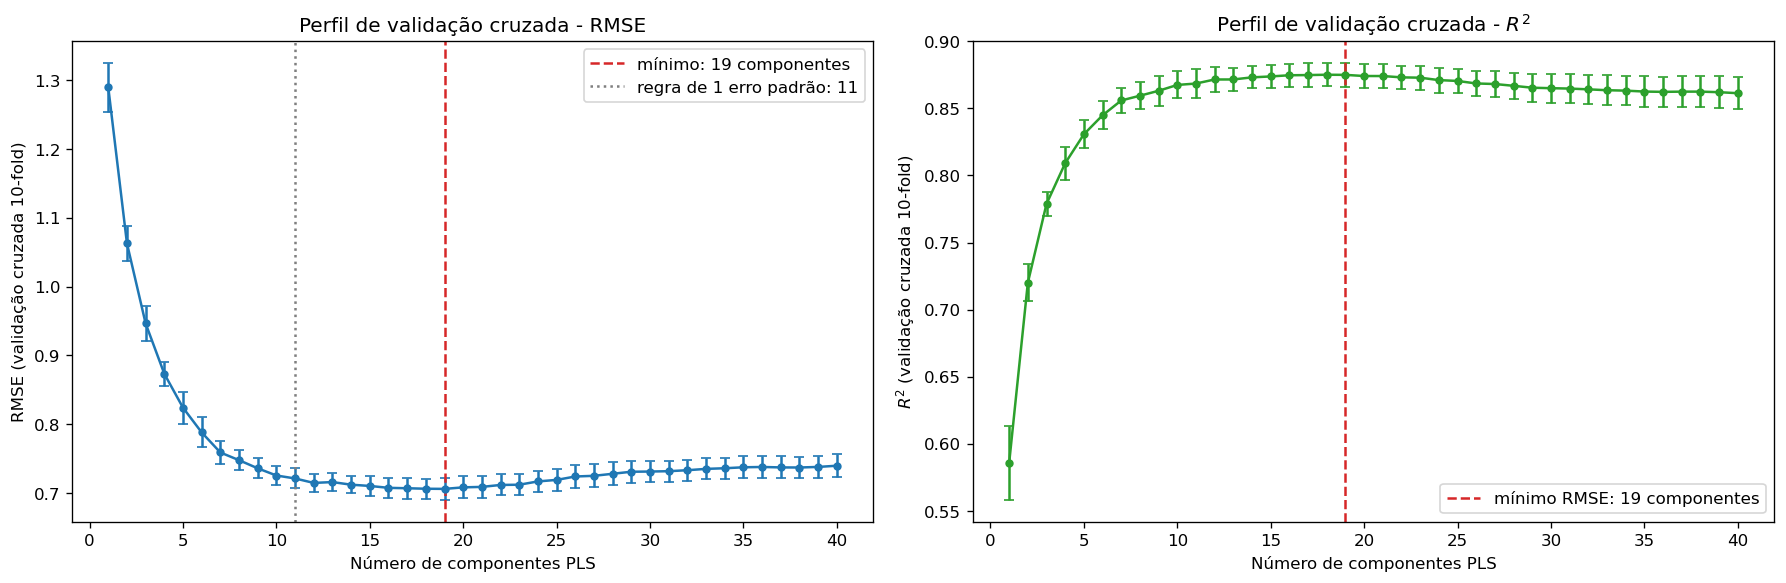
\includegraphics[width=\columnwidth]{pls_perfil_cv.png}
\caption{PLS cross-validation profile of RMSE (left) and $R^2$
(right), with the standard error of the mean over 10 folds.}
\label{fig:pls}
\end{figure}

\begin{figure*}[htbp]
\centering
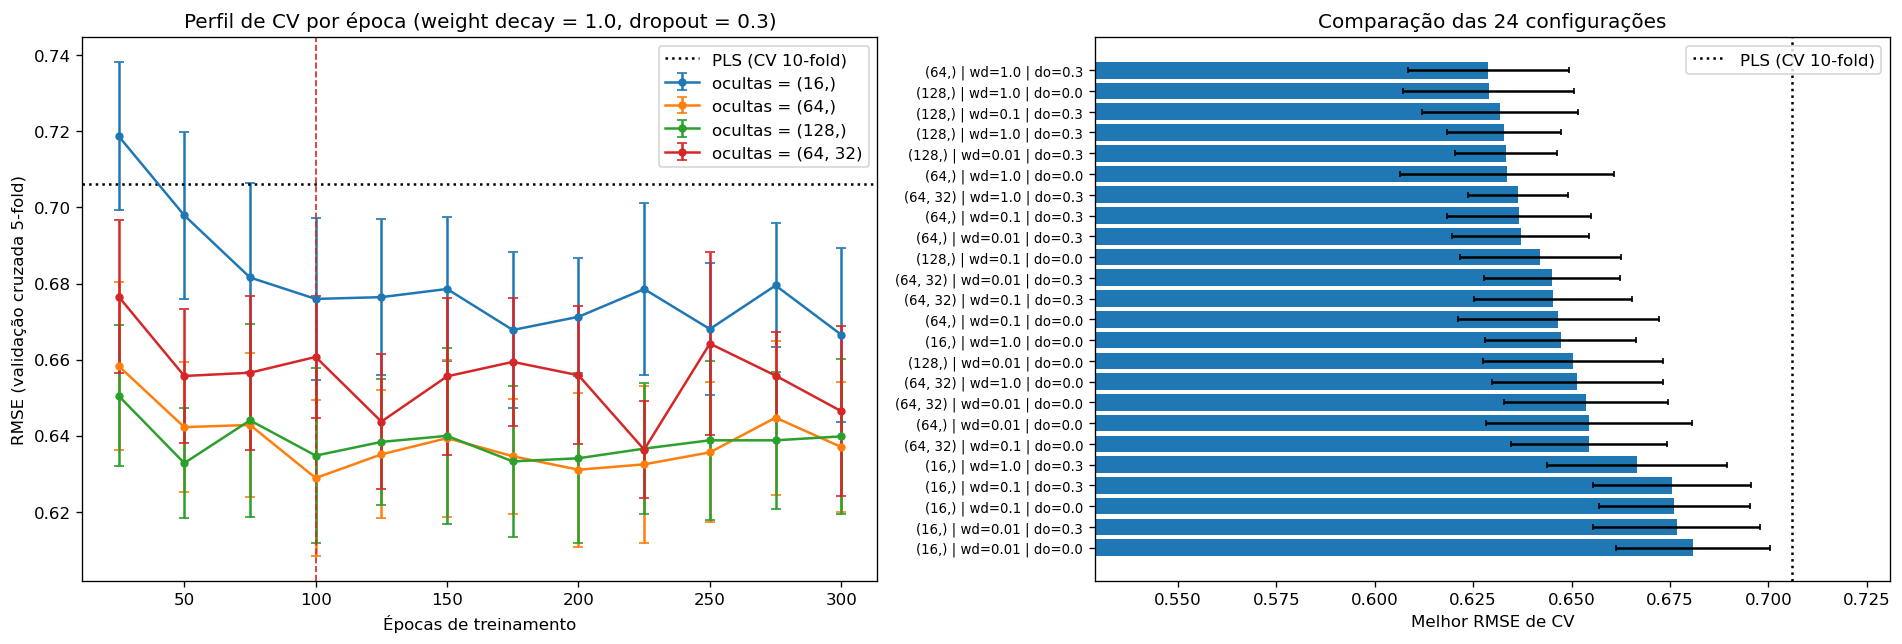
\includegraphics[width=\textwidth]{rn_perfil_cv.png}
\caption{Neural network 5-fold CV: RMSE over the training epochs for the
four architectures with the selected weight decay and dropout (left),
and best RMSE of each of the 24 configurations (right). Error bars show
the standard error of the mean; the dotted line marks the 10-fold CV
RMSE of PLS and the dashed line the selected 100 epochs.}
\label{fig:nn-cv}
\end{figure*}

\begin{figure*}[htbp]
\centering
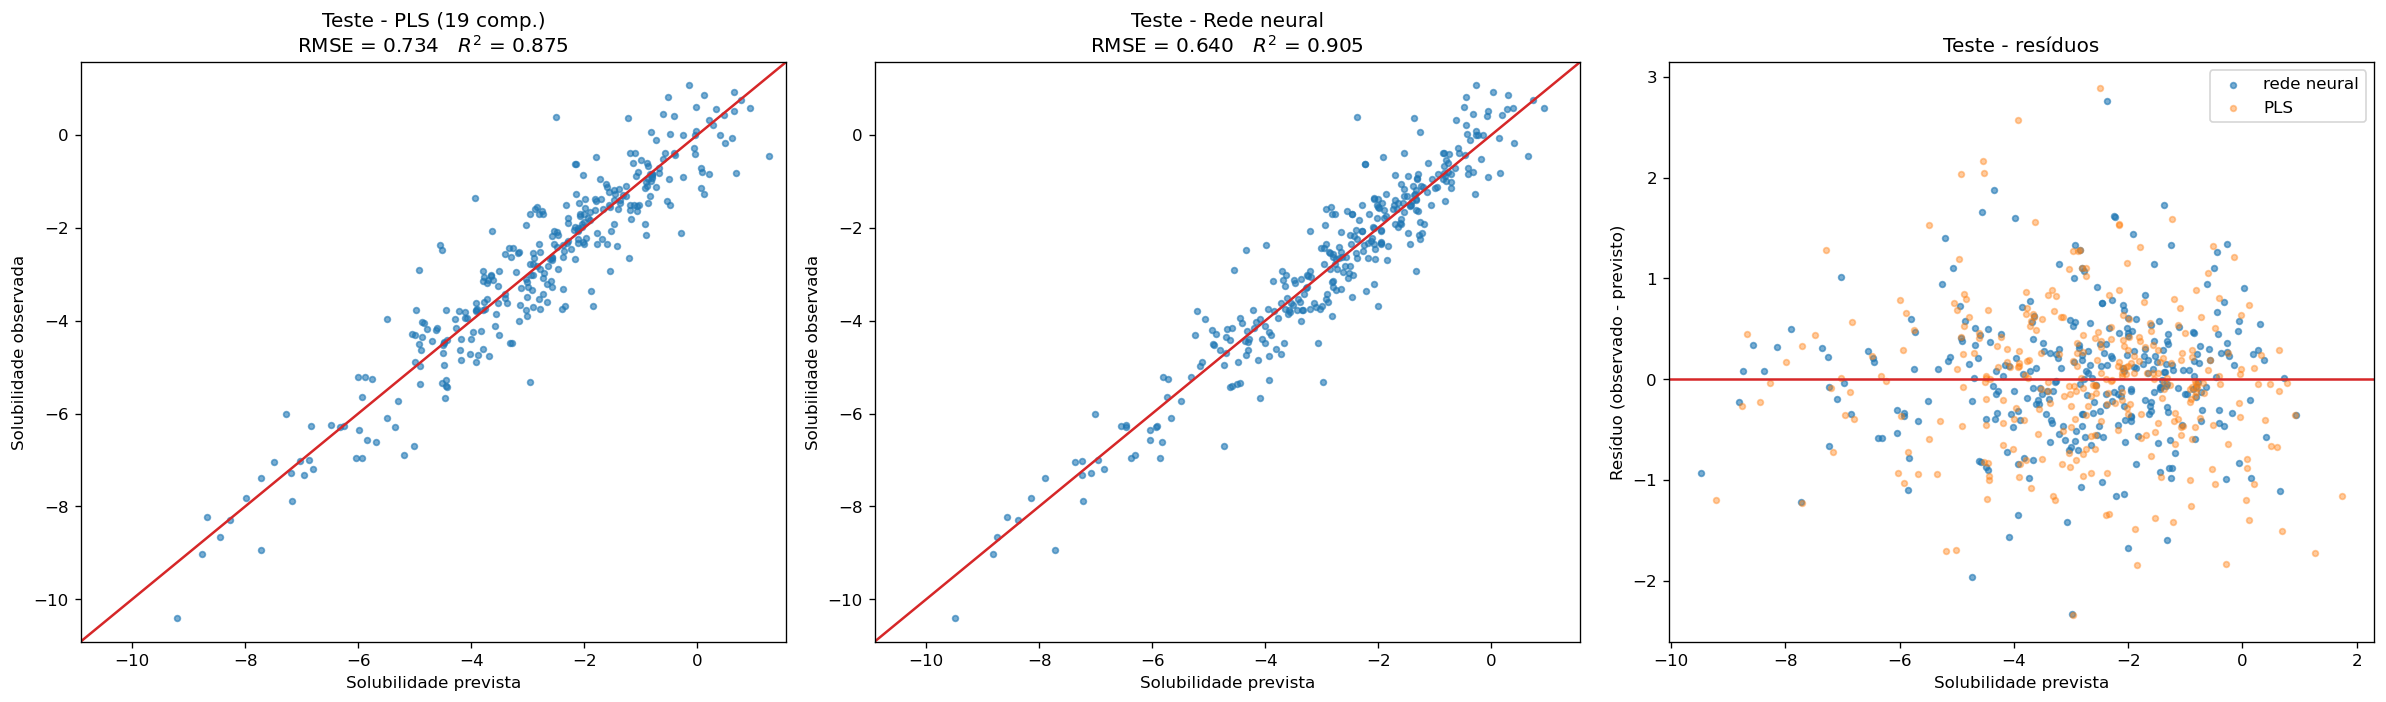
\includegraphics[width=\textwidth]{rn_teste.png}
\caption{Test set: observed against predicted solubility for PLS (left)
and for the neural network ensemble (centre), and residuals of both
models (right).}
\label{fig:nn-test}
\end{figure*}

For the neural network, 5-fold cross-validation selected a single hidden
layer of $64$ units with strong $L_2$ weight decay ($1.0$), dropout rate
$0.3$, and $100$ training epochs, achieving a mean CV RMSE of $0.6289$.
Strong regularisation proved essential to prevent rapid overfitting on
the $951$ training compounds. Fig.~\ref{fig:nn-cv} summarises the
search. With the selected weight decay and dropout, the network with 16
hidden units has the highest error at every checkpoint, and the second
layer of the $(64, 32)$ architecture does not improve on a single
layer. The nine best configurations lie between $0.629$ and $0.637$, all
within one standard error ($0.0204$) of the best, so the error surface
is flat in that region. Averaging the predictions of an ensemble
of $5$ independently initialised networks under this optimal configuration
yielded a test RMSE of $0.6407$ ($95\%$ bootstrap interval
$[0.5729,\ 0.7066]$) and a test $R^2$ of $0.9047$, substantially
improving upon all linear specifications across the entire solubility
range. Fig.~\ref{fig:nn-test} compares the test predictions with those
of PLS: the observed-versus-predicted cloud of the network is tighter
around the diagonal, and its residuals are smaller over most of the
solubility range.

\subsection{Statistical comparison}
\label{subsec:comparison}

Table~\ref{tab:models} consolidates the four models. To assess whether
the differences on the test set exceed the sampling uncertainty of 316
compounds, we use a paired bootstrap \cite{efron1993}. Each of 5000
resamples draws the test compounds with replacement and computes the
RMSE of all models on the same compounds, so that the difficulty of the
resample affects every model alike. For each pair of models,
Table~\ref{tab:pairs} gives the $95\%$ percentile interval of
$\mathrm{RMSE}_A - \mathrm{RMSE}_B$; a positive value favours model
$B$. A difference is significant when the interval excludes zero.
Since there are six simultaneous comparisons, the table also gives the
interval with Bonferroni correction, at an individual level of
$1 - 0.05/6$.

\begin{table}[htbp]
\caption{Consolidated results. CV is 10-fold for the linear models and
5-fold for the neural network. Interval: $95\%$ bootstrap interval of
the test RMSE.}
\label{tab:models}
\centering
\setlength{\tabcolsep}{4pt}
\begin{tabular}{lcccc}
\toprule
Model & CV RMSE & Test RMSE & Interval & Test $R^2$ \\
\midrule
OLS & $0.7279$ & $0.7430$ & $[0.6645,\ 0.8243]$ & $0.8718$ \\
Ridge & $0.6862$ & $0.7175$ & $[0.6457,\ 0.7898]$ & $0.8805$ \\
PLS & $0.7060$ & $0.7337$ & $[0.6595,\ 0.8061]$ & $0.8750$ \\
Neural net. & $0.6289$ & $0.6407$ & $[0.5729,\ 0.7066]$ & $0.9047$ \\
\bottomrule
\end{tabular}
\end{table}

\begin{table}[htbp]
\caption{Paired bootstrap of $\mathrm{RMSE}_A - \mathrm{RMSE}_B$ on the
test set (5000 resamples)}
\label{tab:pairs}
\centering
\setlength{\tabcolsep}{4pt}
\begin{tabular}{lccc}
\toprule
$A$ $-$ $B$ & Diff. & $95\%$ interval & Bonferroni interval \\
\midrule
OLS $-$ Ridge & $0.0255$ & $[-0.0075,\ 0.0593]$ & $[-0.0195,\ 0.0706]$ \\
OLS $-$ PLS & $0.0093$ & $[-0.0248,\ 0.0455]$ & $[-0.0366,\ 0.0573]$ \\
OLS $-$ NN & $0.1023$ & $[0.0524,\ 0.1538]$ & $[0.0322,\ 0.1715]$ \\
Ridge $-$ PLS & $-0.0162$ & $[-0.0350,\ 0.0020]$ & $[-0.0425,\ 0.0076]$ \\
Ridge $-$ NN & $0.0768$ & $[0.0416,\ 0.1138]$ & $[0.0268,\ 0.1262]$ \\
PLS $-$ NN & $0.0930$ & $[0.0498,\ 0.1395]$ & $[0.0325,\ 0.1564]$ \\
\bottomrule
\end{tabular}
\end{table}

No difference among the three linear models is significant. Ridge has
the lowest test RMSE of the group, and it beat PLS in $95.8\%$ of the
resamples, but the interval of that pair, $[-0.0350,\ 0.0020]$, still
contains zero, and the same holds for the pairs involving OLS. The test
set therefore does not support ranking the linear models, even though
cross-validation places ridge first.

The neural network is significantly better than each linear model, with
or without the Bonferroni correction. Its test RMSE is lower by
$0.1023$ than that of OLS, by $0.0768$ than that of ridge and by
$0.0930$ than that of PLS, and it won in at least $99.98\%$ of the
resamples in all three pairs. The cross-validated values point the same
way, although they are not strictly comparable, since the network used
5 folds and the linear models 10.

% =====================================================================
% IV. CONCLUSION
% =====================================================================
\section{Conclusion}
\label{sec:conclusion}

Four regression models were fitted to predict solubility from 228
molecular descriptors, with pre-processing and hyperparameters
determined on the training set only. The OLS, ridge, and PLS estimators
and their cross-validation were implemented from scratch and agree with
the built-in functions to numerical precision.

The three linear models reached test RMSE values of $0.7430$ (OLS),
$0.7175$ (ridge) and $0.7337$ (PLS), with $R^2$ between $0.8718$ and
$0.8805$, and the paired bootstrap found no significant difference among
them. Regularisation changed the coefficients far more than the
predictions: ridge reduced the norm of the coefficients from $152.02$ to
$1.48$ while lowering the test RMSE by only $0.0255$.

The neural network reached a test RMSE of $0.6407$ and an $R^2$ of
$0.9047$, significantly better than every linear model, with a reduction
of $10.7\%$ in RMSE against ridge, the best linear model. This indicates
that the relationship between the predictors and solubility is not purely
linear. Since the linear models already explain about $87\%$ to $88\%$ of
the variance on the test set, the relationship appears predominantly
linear with a smaller nonlinear component. These conclusions rest on a
single test set of 316 compounds, as reflected in the width of the
intervals of Table~\ref{tab:models}.

% =====================================================================
% Declaracao de uso de IA. O enunciado permite que os prompts e as
% respostas fiquem num arquivo separado do repositorio, e e la que
% estao, para nao ocupar as 6 paginas do artigo.
\section*{Use of AI Tools}
AI assistance (Anthropic Claude) was used in this work for code
debugging, for verification queries over the cross-validation and
model results, for structuring the text and for checking the
references. The prompts, the responses and the use made of each are
recorded in \texttt{USO\_DE\_IA.md} in the project repository.

% =====================================================================
% REFERENCES
% =====================================================================
\bibliographystyle{IEEEtran}
\bibliography{refs}

\end{document}